\documentclass[11pt]{article}
\usepackage{acl2012}
\usepackage{geometry}
\usepackage{latexsym}
\usepackage{amsmath}
\usepackage{multirow}
\usepackage{url}
%\usepackage[numbers]{natbib}
\usepackage{graphicx}
\usepackage{subcaption}
\usepackage{float}
\usepackage{multicol}
\newgeometry{margin=2.7cm}
\DeclareMathOperator*{\argmax}{arg\,max}
\setlength\titlebox{3.8cm}    % Expanding the titlebox

\graphicspath{{../figures/}}

\title{{\small CS224W Final Project} \\ What is karma? Quantifying online influence and credibility}
\author{Thomas Dimson \\
  {\tt tdimson@cs.stanford.edu}
  \\\And
  Milind Ganjoo \\
  {\tt mganjoo@stanford.edu}
}
\date{}

\begin{document}
\maketitle

\newcommand{\citet}[1]{\cite{#1}}

\section{Introduction}

Many online communities explicitly publicize the concept of \textit{karma} or
\textit{reputation} for users, computed as a sum of positive votes by other members of
the community. These explicit measures are often seen as proxies for more
intangible notions such as \textit{influence} (the ability of a member to
persuade others) and \textit{credibility} (the trustworthiness of the user as an
member of the community). In this paper, we describe the range of network
characteristics, interactions, and temporal factors that affect the accumulation
of karma points. 

In order to confirm our intuitions about influential network characteristics, 
we evaluate our features on datasets that contain an explicit
measure of karma. However, our primary motivation in developing a model that
enables generalization to \textbf{private communities} without a concept
of ``voting'' for users but with an implied network structure. For example, 
our findings can be applied to e-mail interaction graphs to 
determine a private ``karma'' score for members
of an organization, and to subsequently identify users who have high influence
and credibility.

Our paper is organized as follows: we begin by describing prior studies of
interaction networks in Section~\ref{sec:prior}. Afterwards, we discuss 
our collection of data from two disparate online communities: 
\textit{Hacker News} and \textit{Super User}, and the conversion into 
an interaction graph structure. In Section~\ref{sec:model} we 
examine different properties of these networks and
how they relate to karma and reputation. Using our results, we train
classifiers in Section~\ref{sec:eval} that are able to identify high-karma
individuals with an improvement over our baseline measure. Finally, we 
conclude with future directions of research in Section~\ref{sec:conclusion}.

\section{Prior Work}
\label{sec:prior}

Most prior literature focuses on the abstract quality of \textit{influence}.
Both \citet{bakshy2011everyone} and \citet{cha2010measuring} define influence as
the ability to generate cascades on the Twitter graph. The authors use local
feature of users (e.g.\ number of followers, number of tweets, retweets,
mentions) in order to predict the ability for users to generate cascades.

\citet{cha2010measuring} emphasizes the topic-specificity of influence -- they
challenge the notion that there is a common set of ``influentials'' who have
broad-reaching impact on online communities. Instead, they demonstrate that for
many topics, such as political events, there are special interest groups like
bloggers and politicians that see higher retweet and mention scores than the
generally popular Twitter users.

In a very recent paper, \citet{movshovitzanalysis} consider the reputation
scheme on StackOverflow (based on upvotes and accepted answers). They attempt to
identify expert users based on their contribution patterns and use high
reputation users for validation. The authors tried many techniques to improve
their classifier performance including PageRank and an SVD decomposition of
their interaction graphs. Notably, they find that PageRank does not contribute
significantly to their performance and use user features such as number of
answers, questions and question-answer rations in their final random forest
model. They are able to achieve an Area under the Curve of 81\% when classifying
users with reputations of more than 2400.

\section{Datasets}

In this paper, we will be focusing on two relatively large internet communities:
\textbf{Hacker News} and the \textbf{StackExchange} family of websites. On
Hacker News, users submit technology-related stories as \textit{submissions}
which other users use as an anchor to threaded discussions.  A user's
\textit{karma} is computed as a sum of up-votes to their stories and comments.
The StackExchange family of websites are question-and-answer sites where a user
will post a question and solicit answers from the community. A user's
\textit{reputation} is a weighted sum based on the number of their questions and
answers that are accepted and voted helpful by the community.

Our choice of online communities was deliberate: one on hand, we have the
\emph{discussion-focussed}, eccentric community of Hacker News, and on
the other we have a focused question-answering website. The
contrasting between the two networks provides for some interesting
observations, which we describe in Section~\ref{sec:model}.

Gathering data for Hacker News came with many challenges: there is no published
dump of Hacker News data, and no official API. Fortunately, the creator of
ThriftDB has created HNSearch\footnote{\url{https://www.hnsearch.com/}} as a
technology demo for his database. Over the course of a week, we
extracted JSON files for every comment, submission and user on Hacker News by
repeatedly querying the API\@. To our knowledge, ours is the only complete dump
of this data available on the internet.

Collecting data for the StackExchange family of websites was easier.
An anonymized data dump of the entire series of websites is released every three
months\footnote{http://www.clearbits.net/creators/146-stack-exchange-data-dump}
in XML format. We wrote a Python script to parse the XML data and extract
relevant fields. We chose to focus on \textbf{Super User} website since it
has a manageable amount of data.

We converted our dataset into an interaction graph by 
collecting $(\text{replier}, \text{parent poster})$. A summary of our datasets is
available in Table~\ref{tab:graphstats}. As a final step, we divided each
dataset into train, validation and test sets at a 70\%/15\%/15\% split.

\subsection{Karma distribution and statistics}

\begin{figure*}[t]
\centering
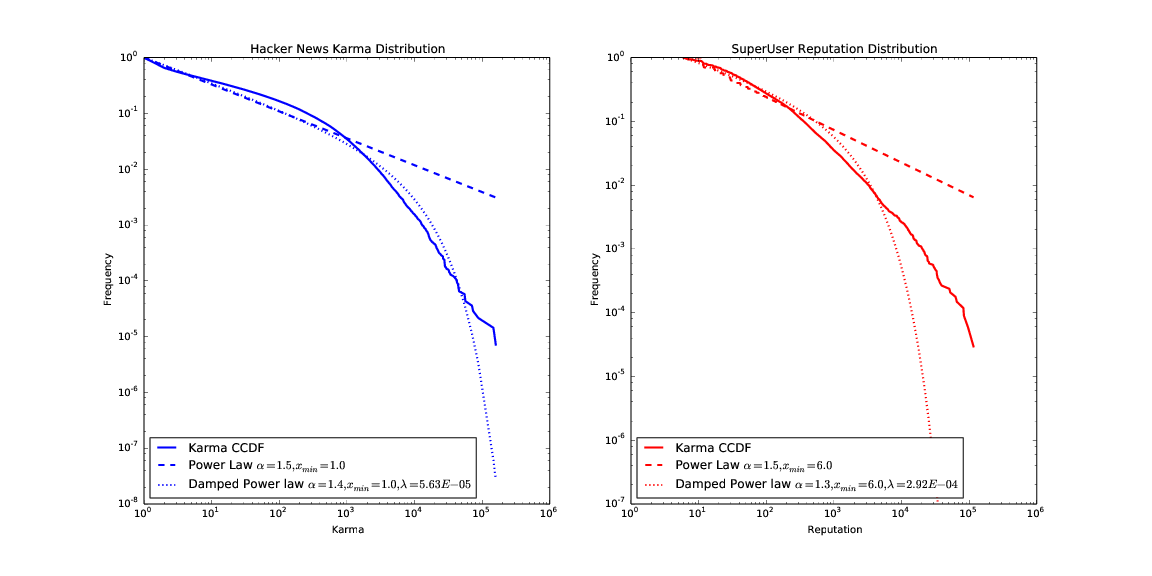
\includegraphics[width=0.95\linewidth]{powerlaws-png}
\caption{Karma distributions in our datasets with fitted power law distributions}
\label{fig:powerlaws}
\end{figure*}

Figure~\ref{fig:powerlaws} shows a fitted power law plot for our reputation and
models. Both models have an $\alpha$ coefficient near 1.5 and $x_{\text{min}}$
near the origin. Notably, a damped power law is a better fit than a power law on
our Hacker News distribution and the reverse is true for our Super User
reputation karma distributions. The reason for this could be that Hacker News,
being an older community (c. 2007), has a few early adopters with incredibly
high karma that deviate from the normal power law. On the other hand, Super User
is relatively new (c. 2011), and comprises users that split off of the existing
StackOverflow community, who follow a more traditional power law.

\begin{table*}[t]
\begin{center}
\begin{tabular}{| r | l l |}
\hline
& \textbf{Hacker News} & \textbf{Super User} \\
\hline
Users (Nodes) & 175091 & 190781 \\
Replies (Edges) & 2747966 & 266673 \\
Average Karma / Reputation & 131.8 & 83.1 \\
Largest SCC Fraction & 43\% & 3.8\% \\
Largest WCC Fraction & 63\% & 46\% \\
\hline
\end{tabular}
\end{center}
\caption{Graph statistics for our implied interaction graphs}
\label{tab:graphstats}
\end{table*}

Aligning with our karma distributions, Table~\ref{tab:graphstats} shows
interaction graph statistics for both communities. Although they are roughly
commensurate in users, Hacker News has an order of magnitude more edges in the
graph due to the threaded nature of discussions. The disparity between the
communities increases when we begin to look at strongly connected components
(SCCs): over 40\% of Hacker News members are part of their largest SCC while
only 3.8\% of Super User members are part of their largest SCC\@. This reflects
the fact that members on a Q\&A site have fewer ``spanning'' conversations,
preferring to stick to their comfort zones in both questions and answers (there
are no reputation points for comments on any of the Stack Exchange websites). As
a result, the graph structure is much looser. The largest weakly connected
component (WCC) is an order of magnitude larger than the largest SCC on Super
User and it suggests distinct roles of \textit{questioners} and \textit{answers}
with relatively little overlap. We explore the consequences of the graph structure
differences in Section~\ref{sec:model} and during evaluation in Section~\ref{sec:eval}.

\section{Model and Features}
\label{sec:model}

Armed with the knowledge of our karma distributions we look more closely at network
characteristics that could serve for predictive purposes. We describe
both features that worked well and those that not perform as well 
as expected.

\subsection{Karma Cliques and Preferential Attachment}
\label{sec:karma_cliques}

One model that seems intuitive is that high reputation users tend to attach to
other high reputation users, forming so-called \textit{karma cliques}. We
initially tested this hypothesis by logarithmically-bucketing karma/reputation
and computing \citet{newman2003mixing}'s assortativity over karma levels. This
yields relatively low assortativity of $0.015$ and $0.040$ on Hacker News and
Super User respectively.

Beyond correlations, Figure~\ref{fig:karma_cliques} shows a scatter plot of the
average neighbor karma. In both networks, the mean average neighbor
karma remains relatively constant at all karma levels, although the variance
shrinks as karma increases.  Super User's plot is dramatically different than
Hacker News: there are two distinct ``clusters'' based in inbound/outbound neighbor
karma. We see that the inbound reputation (people answering this
post) tends to be much higher than the outbound karma (the questioner's karma).
This suggests two distinct roles on Super User: the questioners and the answers.
Hacker News does not appear to have this distinction.

Based on our plots and our relatively low assortativity score between karma, we
saw \textit{no evidence of preferential attachment between similar-karma nodes}
on either network.

\begin{figure*}[t]
\centering
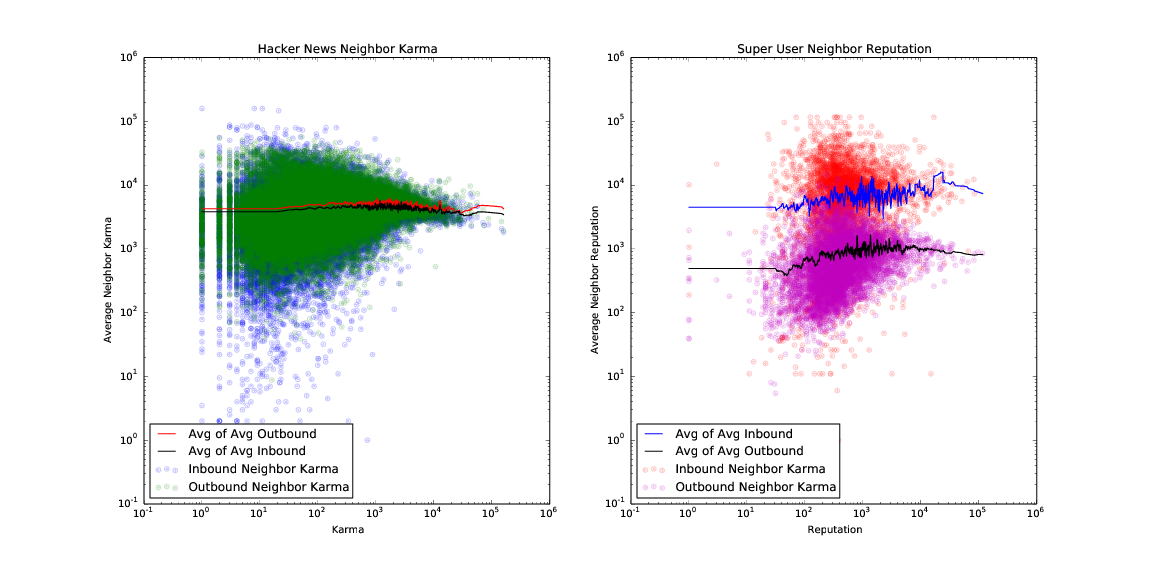
\includegraphics[width=\linewidth]{karma_cliques-png}
\caption{Scatter plot of average neighbor karma against the anchor node's karma. 
The lines represent the mean average neighbor karma at a given karma level.
Neighbor karma variance appears to shrink with larger anchor karma values.}
\label{fig:karma_cliques}
\end{figure*}


\subsection{Node Features}
\begin{figure*}[t]
\centering

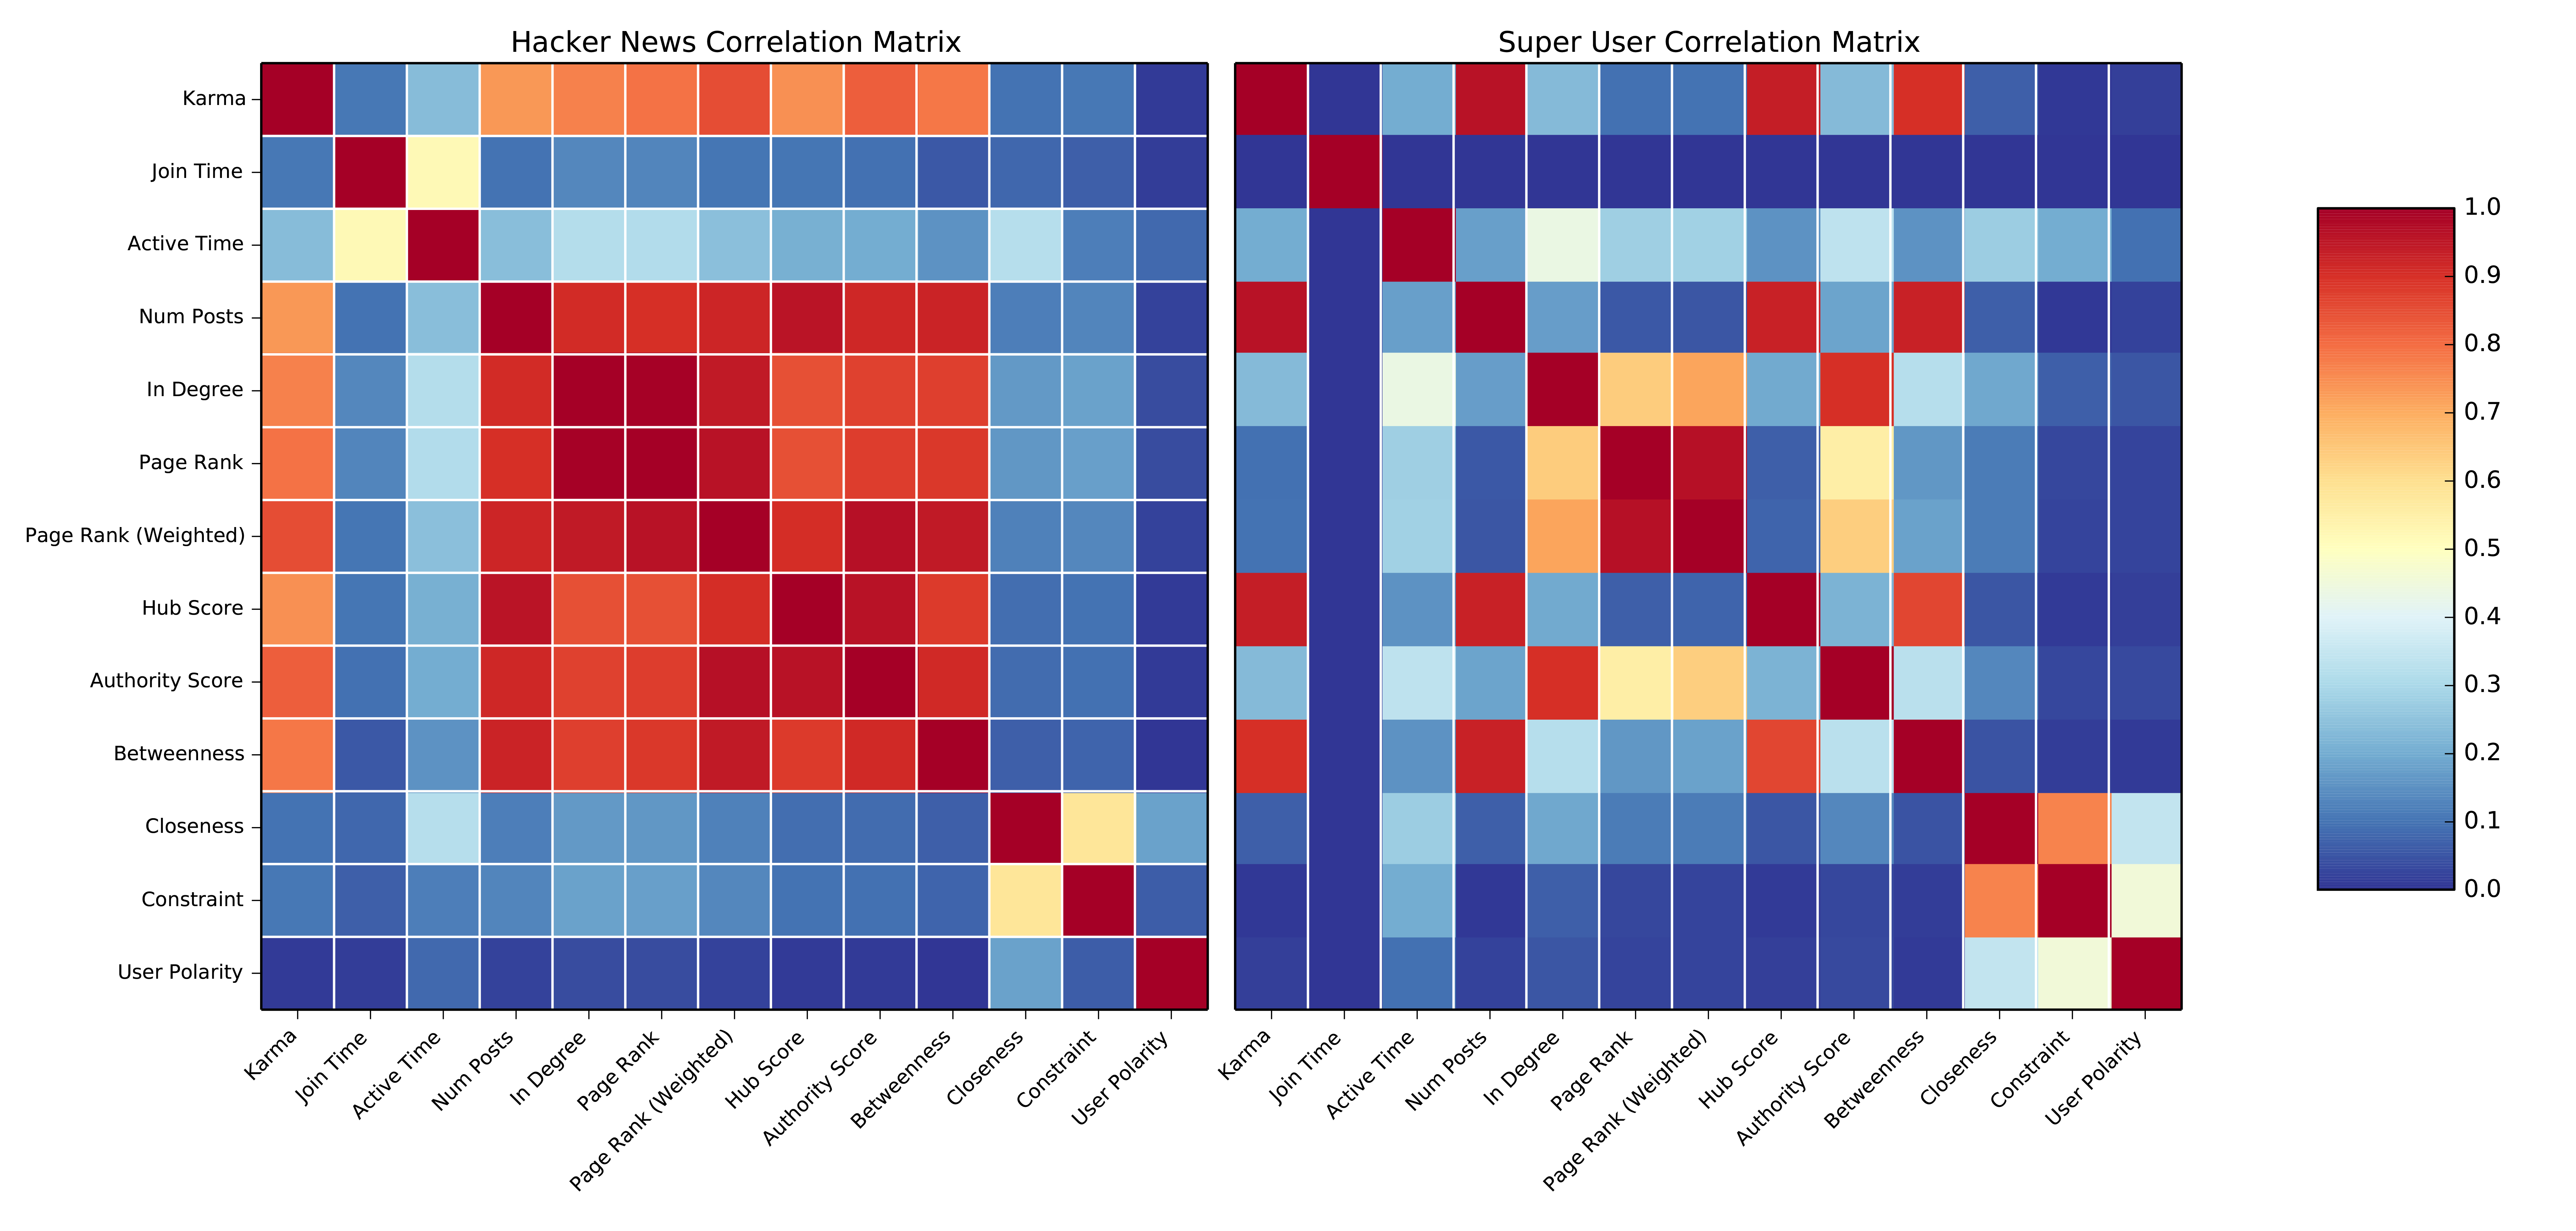
\includegraphics[width=\linewidth]{correlation-png}
\caption{Pearson's correlation coefficient matrix for some of our features.
Notice the dramatic difference in correlations when switching between 
Hacker News and Super User.}
\label{fig:correlation}
\end{figure*}
Based on intuition from \citet{movshovitzanalysis}, we construct a baseline
from two features: the number of replies made by a user since joining the website,
and the length of time since the user joined (in seconds). The authors' work
suggests that these two features are strongly correlated to reputation on Stack
Overflow, and we find a similar result on Super User. As discussed in 
Section~\ref{sec:classification}, the baseline features seem less 
important on Hacker News.

\subsection{Network Features}

\subsubsection{Centrality: PageRank, HITS, betweenness and closeness}
\label{sec:centrality}

By definition, centrality measures correspond to a node's importance in the
graph and it is natural to assume that karma and reputation are proxies for
importance. In our analysis we looked at degree centrality, variants of
PageRank~\cite{page1999pagerank}, Hubs and Authorities
(HITS)~\cite{kleinberg1999authoritative}, betweenness and closeness. As we will
see, our most (linearly) predictive features correspond to centrality in
network-specific ways.

Our analysis of Hacker News supports a blunt hypothesis: members of the Hacker
News community are \textit{contributors}, and contributions come in the form of
replying and receiving replies equally. In fact, the correlation coefficient
between out-degree (number of posts) and in-degree is $0.995$. We then ask
\textit{are all contributors are equal?}. To answer this, we ran two variants of
PageRank: vanilla and a version where transition probability is proportional to
the number of replies. Our weighted variant is our most linearly predictive
feature for karma ($\rho = 0.85$ Vs. $\rho=0.79$ vanilla).
Figure~\ref{fig:correlation} shows that with the exception of closeness, other
centrality measures are highly correlated with karma on Hacker News.  
Our hub score correlation is slightly lower than authority score and suggests 
a slight bias for high quality content over replying to other contributors.

Centrality measures on Super User further support the evidence distinct
``questioner'' and ``answerer'' roles noted in Section~\ref{sec:karma_cliques}.
Unlike Hacker News, Figure~\ref{fig:correlation}, shows no clear linear
correlations between our centrality measures. In particular, PageRank and
authority scores do not correlate at all to reputation. In contrast,  in-degree 
and hub score are directly related to reputation. Since edges are directed from answerer
to poster, it seems that on Super User
\textit{it doesn't matter who answers you, it matters whether you answer others}.

Although betweenness also appears to play a role on Super User, we see that
both hub score and betweenness both correlate with the out-degree of nodes.
We believe this is because the weak component structure outlined in 
Table~\ref{tab:graphstats}. Obviously, more shortest paths will pass through a
node of high out-degree in a network that is primarily weakly connected.

\begin{figure}[h]
\centering
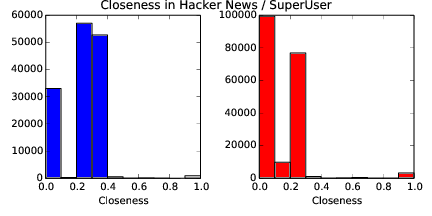
\includegraphics[width=\linewidth]{closeness-png}
\caption{Closeness distribution in both networks}
\label{fig:closeness}

\end{figure}

Figure~\ref{fig:closeness} shows a histogram of another measure of centrality --
closeness, or the inverse of the sum of distances from a node to all other
nodes. For Hacker News, nodes are closer together in terms of shortest paths 
(closeness between $0.3$ and $0.4$ for the majority of values), while on Super User nodes
are further away (near zero closeness for most values). This appears to reflect
the stronger sense of community on Hacker News, and the consequent ease of
information spread as a result.

\subsubsection{Network constraint}
\label{sec:constraint}

\begin{figure}[h]
\centering
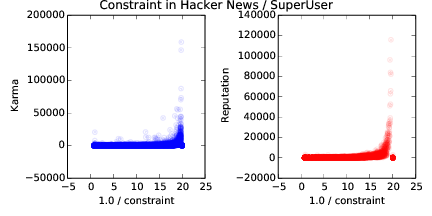
\includegraphics[width=\linewidth]{constraint_correlation-png}
\caption{Scatter plot between $\frac{1}{\text{constraint} + 0.05}$ and karma}
\end{figure}

We also compute the network constraint for each node in both networks and plot
the constraint values against karma. We notice empirical evidence of some 
inverse correlation between the two for both networks, i.e that high karma and
reputation score users have lower constraint scores. This is in line with the
intuition that a high karma person would tend to have interactions across a
large, disparate set of users. As we discuss in Section~\ref{sec:eval}, low constraint
appears to be a necessary but not sufficient property for high karma: there are
many users with low constraint and low karma.

\subsection{Textual Features}

Beyond weight, each edge in our interaction graphs are augmented with the
\textit{text} corresponding to the reply that was made. One would expect 
text (i.e.\ insightful replies and helpful answers) to play the largest role 
in influence and karma. As we'll see below, this isn't necessarily the case.

\subsubsection{Sentiment Analysis}
\label{sec:sentiment}
\begin{figure}[h]
\centering
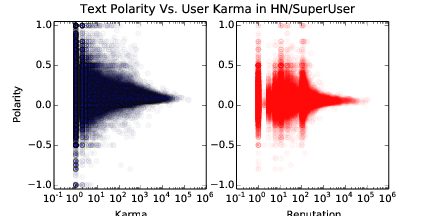
\includegraphics[width=\linewidth]{text_polarity-png}
\caption{Sentiment scatter plot against karma / reputation}
\label{fig:sentiment}
\end{figure}

Figure~\ref{fig:sentiment} shows a scatter plot comparing user karma
against user sentiment. We compute user sentiment by concatenating all
their replies together and running Python's pattern module \citet{de2012pattern}, 
which implements sentiment classification using a fixed sentiment lexicon.  Both
Hacker News and Super User have a slight positive bias (mean polarity of 0.11 and
0.07 respectively). Plotted on a log scale, we see a linear envelope enclosing
the means. As such, while polarity is not linearly correlated with karma,
\textit{it pays to toe the line}: there are no examples of extremely high karma
users that have large polarity deviations. Furthermore, all examples of
highly-biased users occur towards the lower end of the spectrum. Although
sentiment analysis is never perfect, it provides a quick way of ruling out users
as being big influencers.

\subsubsection{Topic Modelling}

Another axis of textual analysis is clustering the content of posts in terms of
broad categories or topics. To this end, we performed Latent Dirichlet
Allocation (LDA) \cite{blei2003latent} across user text. We wished to answer two
questions: \textit{are broader knowledge bases associated with higher karma}?
and \textit{are there different karma models across different topics}?

\begin{figure}[h]
\centering
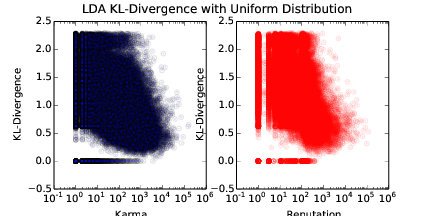
\includegraphics[width=\linewidth]{lda_kl-png}
\caption{User text KL-Divergence with uniform distribution Vs. Karma}
\label{fig:lda_kl}
\end{figure}

In Figure~\ref{fig:lda_kl}, we try to measure whether having a broad knowledge
base is associated with higher karma. To this end, compare the KL-divergence of
a user's topic distribution with that of the uniform distribution and plot it
against reputation/karma. Plotted on a log scale we see a similar ``bow''
pattern between the two networks, showing a wide variance in KL-divergence with
a trend downwards for high reputation. Although our evidence is much weaker than
that of sentiment in Section~\ref{sec:sentiment}, this pattern shows that
``important people'' in the communities tend to have broad knowledge bases which
we can exploit when trying to classify people.

The variance in KL-divergences of Figure~\ref{fig:lda_kl} suggests that there
are different karma models across topics. As a coarse method of evaluation, we
examined the measure of average expected karma, which we defined per topic $t$
as
\begin{align*}
AEK_t = \frac{1}{n} \sum_{\text{node} i}^n P_t(i) * \text{Karma}(i)
\end{align*}

Per-topic, these measures can be compared with a baseline uniform average
expected karma (15 for hacker news and 8 for Super User). For Super User, we
notice a wide variance in the expected reputation across topics: the AEK lies in
the interval $[2.4, 13.3]$ depending on the topic. The lowest AEK values come
with topic 2 (2.4 AEK), associated with words such as \textit{column, excel
cell, table and formula}. We can contrast this to the
largest AEK value with topic 8 (13.3 AEK) associated with words such as
\textit{memory, support, number, process, performance and hardware}. Thus, on
Super User more reputation mass is associated with answering certain classes of
problems: people tend to reward performance tips more than Microsoft Excel tips.
Since the site bills itself for ``power users'', this matches our intuition for
subjects on the site.

The Hacker News view of topic is less dramatic than Super User with values lying
on the interval $[10.4, 23.2]$. Here, the lowest topic (number 3 at 10.4 AEK) is
associated with words such as \textit{energy, english, countries, europe,
water}. The highest topic (number 0 at 23.2 AEK) is associated with words such
as \textit{startups, customer, marketing, revenue, founders}. As the Hacker News
originated with a startup incubator this match seems to make intuitive sense:
more karma mass lies in topics central to the site.

Building on the intuition of different expected karma, we tried running a variant of 
PageRank where the transition probability is replaced with the topic probability of 
the reply. Intuitively, this would allow us to identify ``topic experts'' in the 
community who have high karma. Unfortunately, the rank vectors were highly correlated
with each other and didn't appear to provide much new information. The correlation is 
a reflection of high-karma users having the broad knowledge bases identified in 
Figure~\ref{fig:lda_kl}.


\section{Evaluation \& Results}
\label{sec:eval}

We evaluated our model and statistics described in Section~\ref{sec:model}
within a \textit{karma prediction} task. Essentially, we remove the value of
karma from our dataset and then try to reconstruct it using left-over network
information. This allows us to validate our features and see how well they might
generalize to networks without an explicit notion of karma. In addition to
determining the exact value of karma (Section~\ref{sec:regression}) we also
identified high-karma users in our dataset via classification
(Section~\ref{sec:classification}). The results of running prediction on 
our validation set are summarized in Table~\ref{tab:eval}. 
\begin{table*}
\centering
\begin{tabular}{|r| l l l | l l l|}
\hline
      & \multicolumn{3}{c |}{\textit{Hacker News}} & \multicolumn{3}{c|}{\textit{Super User}}  \\
\textbf{Model} & \textbf{AUC} & \textbf{RMSE} & $\textbf{R}^2$ &
\textbf{AUC} & \textbf{RMSE} & $\textbf{R}^2$ \\
\hline
Baseline & 0.63  & 563.17 & 0.55 & 0.75 & 187.35 & 0.96 \\
Weighted PageRank & \textbf{0.76} {\tiny (logit)}  & 484.44 & 0.67 & 0.20 & 998.87  & 0.00 \\
HITS & 0.72 {\tiny (logit)} & 618.16 & 0.62 & 0.68 {\tiny (logit)} & 292.60  & 0.91 \\
Constraint & 0.57 & 642.56 {\tiny(RF)} & 0.41 & 0.60 & 396.51 {\tiny(RF)} & 0.84 \\
Textual & 0.19  & 825.36 & 0.04 & 0.51 & 987.82 & 0.01 \\
LDA Rank & 0.75 {\tiny (logit)} & 502.13 & 0.64 & 0.31 & 991.31 & 0.00 \\

Baseline+Constraint & 0.69 & 562.63 & 0.55 & 0.71 & 187.17 & 0.96 \\
Baseline+Textual & 0.64 & 561.79 & 0.55 & 0.72 & 187.32 & 0.96 \\

All Features & 0.75 & \textbf{483.1} {\tiny(RF)} & \textbf{0.67} {\tiny(RF)} &
\textbf{0.78} & \textbf{184.89} & \textbf{0.97} \\
\hline
\end{tabular}

\caption{Evaluation results for regression and ``famous'' classification for
various feature combinations. AUC is the area under the precision/recall curve
for the high karma/reputation prediction task.
Except where specified, classification results use a Random Forest classifier
while regression uses ordinary least squares.}
\label{tab:eval}

\end{table*}

\subsection{Famous Prediction}
\label{sec:classification}

\begin{figure}[h]
\centering
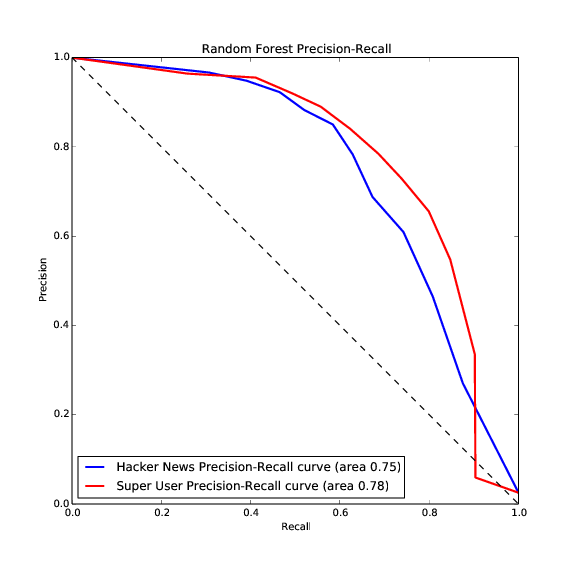
\includegraphics[width=\linewidth]{classification_pr_curve-png}
\caption{Precision/Recall Curve for our best high-karma classifiers}
\label{fig:classification}
\end{figure}

In our famous prediction task, we predict users that
pass a certain threshold of karma. Our power law distributions in
Figure~\ref{fig:powerlaws} suggests that we will have infinite moments, so we
chose to set a threshold based on the ``top 2.5\%'' of users (have more karma
than 97.5\% of others) instead of looking at standard deviations. This
corresponds to thresholds set 1308 and 350 for Hacker News and Super User
respectively.  To capture non-linearities in the data we use a random forest
classifier and evaluate our performance by the area under precision/recall
curve. We also ran a logistic regression classifier to rule out some 
learning biases.

We use a baseline model taken from \citet{movshovitzanalysis}, attempting to
classify famous users by the length of time they have been members and the
number of posts they've made. As Table~\ref{tab:eval} shows, the performance on
both datasets is quite respectable: we can get up to 63\% AUC on HN and 75\% AUC
on SU by looking at just these features.

In our analysis, we are less interested in raw performance and more interested in 
simple features that might generalize
to graphs without an explicit measurement of karma. As such, we also built classifiers
with more limited subsets of our features to determine how well they perform. Of particular note,
we can achieve our \textit{best} famous prediction performance (0.76 AUC) 
on Hacker News by performing PageRank on a weighted version of the graph and training
a logistic regression classifier on the result. Other link analysis centrality measures 
appear to have similar performance, indicating that \textit{the primary indicator of karma 
is centrality} on Hacker News.

In contrast, weighted PageRank gives terrible performance on our Super User dataset
(0.20 AUC vs \. 0.78 best). As we noted in Figure~\ref{fig:correlation}, it matters
more what kind of questions you \textit{answer} on Super User than those you 
\textit{ask}: indicating a measure the hub score would perform better than
the authority score. Table~\ref{tab:eval} shows that HITS can boost performance
on Super User up to 0.68. Still, all network analysis measures on Super User 
are outperformed by looking only at our baseline of number of posts and the length
of time. This may be an indication of Super User being a newer community, and the
way reputation is assigned (rewarding quantity of answers more than quality of answers).
It seems quite plausible that reputation in the early days of a community is mostly
distributed amongst early adopters.

When looking at textual features (sentiment, LDA) alone, our classifier does better than random 
but not particularly well on either network (0.19 and 0.51 AUC). Remarkably, content
seems to have less effect than the network structure around replies. Similarly, the LDA Rank model 
described in Section~\ref{sec:eval} has similar performance to our weighted PageRank baseline. 
This shows that it is less important to be a \textit{topic expert} than it is to be a general
\textit{expert}.

All of our features seem to have linear and non-linear dependencies between them. When we combined
them into a big classification model, Super User classification scores improved mildly (to 0.78 AUC)
but the Hacker News score is slightly worse than just using weighted PageRank alone. The performance
further suggests that network centrality is the most important feature in karma.

\subsection{Karma/Reputation Regression}
\label{sec:regression}
% Needs expansion
\begin{figure}[h]
\centering
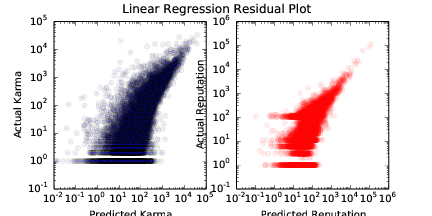
\includegraphics[width=\linewidth]{residuals-png}
\caption{Log-log plot of predicted Vs.\ actual karma/reputation values}
\label{fig:residuals}
\end{figure}

In our regression task, we attempt to predict karma values \textit{directly}
utilizing the same dataset as used in our famous prediction task. Our
improvement patterns mostly match that of our classification although our scores
(as quantified by RMSE) are modest. Figure~\ref{fig:residuals} shows a plot
of predicted karma/reputation Vs.\ actual karma/reputation. Here, we can see that
while we are relatively successful at identifying ``famous'' individuals, we are
much less successful with lower-karma users.

Throughout our regression task, we compared two models of regression: ordinary least
squares  and random forest regression. Table~\ref{tab:eval} shows the performance of 
the best classifier - typically ordinary least squares with the exception of network
constraint. As we discussed in Section~\ref{sec:constraint}, constraint is not
a linear feature - having low constraint seems to be necessary but not sufficient
for having high karma. This is reflected in our performance: significantly better
than random on both networks but also outperformed by other features.

\subsection{Rank correlation}

In addition predicting reputation and karma scores for users we can also
use regression to order the set of users in each network. To quantify
our ordering, we calculating the Kendall rank correlation 
coefficient ($\tau$) between gold and predicted ranks. Our users are split into two sets:
all users and those that are ``famous'' in our gold set as identified in 
Section~\ref{sec:classification}. Table~\ref{tab:kendall} summarizes our findings.

\begin{table}[h]
\setlength{\tabcolsep}{2pt}
\small
\centering
\begin{tabular}{|r| c | c | c | c |}
\hline
      & \multicolumn{2}{c |}{\textit{Least-squares}} &
      \multicolumn{2}{c|}{\textit{Random forest}}  \\
\textbf{Model} & \textbf{All} & \textbf{Famous} &
\textbf{All} & \textbf{Famous} \\
\hline

Baseline (HN) & 0.42  & 0.31 & 0.51 & 0.28 \\
Baseline (SU) & 0.29  & 0.50 & 0.29 & 0.50 \\
All features (HN) & 0.51  & 0.36 & 0.61 & 0.35 \\
All features (SU) & 0.28  & 0.54 & 0.38 & 0.57 \\

\hline
\end{tabular}

\caption{Value of Kendall rank correlation coefficient $\tau$ for our models.
We calculate the value of $\tau$ over all users and ``famous'' users separately.}
\label{tab:kendall}

\end{table}

According to our table, we are better at ranking users when using random
forest regression as than to least-squares, which is consistent with the
analysis in Section~\ref{sec:regression}. Interestingly, we
notice that we are better at ranking the entire set of users on Hacker News, but
on Super User we are better at ranking the famous users. Our hypothesis is that
Super User's reputation only starts to differentiate itself for famous users because
there are a lot of low reputation users who ask and answer very few questions,
or very niche questions. So, it is harder to be ``noticed'' on Stack Overflow 
without quality answers. On Hacker News, where every comment gets attention, we 
find granularity in karma values of less-famous users as well.  Conversely, because
of the tighter community structure of Hacker News, famous users are relatively
close together in scores, and therefore harder to differentiate. This effect was
observed in the exponentially damped karma distribution of Hacker News (Figure~\ref{fig:powerlaws}).

\subsection{Prediction examples}
To demonstrate our results, we selected the top 10 gold users 
and top 10 predicted users for karma and reputation on both networks
and empirically compared their actual scores with predicted scores. 
7 of the highest gold users on HN and 8 of the highest on SU 
are also predicted as top-10 by us.

Some scores are particularly interesting -- on Hacker News, we
predict a score of 25995 for user \texttt{petercooper} with actual karma 26332 --
a difference of 1.2\%. On the other hand, we predict a value of 6140 for user
\texttt{nickbb}, while their actual karma is 27593. However, on closer inspection
we find that 88.92\% of their karma score comes from submissions rather than
comments. We were unable to incorporate submissions since they do not have
a clear mapping into an interaction graph. Overall, we observe a median difference of
20.80\% in the Hacker News top ten. On Super User, where all reputation is earned 
through questions and answers, we observe a median
difference of 27\% between predicted and actual scores.

\section{Conclusion}
\label{sec:conclusion}

In this paper, we discuss the network factors affecting \textit{karma and reputation}
in two disparate communities: Hacker News and
Super User. The network structure of these communities is quite different, with
Hacker News having users that tie together others into a large strongly
connected component whereas Super User users fall into roles of ``questioners''
and ``answerers'' that force the graph to be more disconnected. Despite the
differences in structure, we find that network \textit{centrality} measures are
the strongest indicators of a node's karma or reputation. Beyond centrality and
almost without exception, high karma users have a large number of ``weak ties''
(as measured by \textit{constraint}) and act as bridges between different parts
of the network (large \textit{betweenness}). We find that content plays less of a role
in karma: although there are some differences in karma models
between \textit{topics} of discussion, most high-karma users have broad
knowledge bases with neutral sentiment. 

We recognize a certain amount of randomness inherent in the voting patterns 
of both networks that scores do not depend on contribution alone. Thus, 
the ``perfect classifier'' may be  impossible to create. However, the efficacy 
of centrality measures  is undoubtedly useful in the prediction task. 
The features we developed can be applied to the broader influence-identification 
task in networks without an explicit notion of karma. We are looking forward
to analyzing these private datasets in future work.

\bibliography{report}{} \bibliographystyle{acl2012}

\end{document}
